In this section, we describe how the domain decomposition and the
exchange of particles are implemented in FDPS. We used the
multisection method
\citep{2004PASJ...56..521M} with the so-called sampling
method \citep{Blackston:1997:HPE:509593.509597}. The multisection
method is a generalization of ORB (Orthogonal Recursive Bisection). In
ORB, as its name suggests, bisection is applied to each coordinate
axis recursively. In multisection method, division in one coordinate
is not to two domains but to an arbitrary number of domains. Since one
dimension can be divided to more than two sections, it is not
necessary to apply divisions many times. So we apply divisions only
once to each coordinate axis. A practical advantage of this method is
that the number of processors is not limited to powers of two.

Figure~\ref{fig:decomposition} illustrates an example of the
multisection method with $(n_x, n_y, n_z)=(7,6,1)$. We can see that
the size and shape of subdomains show large variation. By allowing
this variation, FDPS achieves quite good load balance and high
scalability. Note that $n=n_x n_y n_z$ is the number of MPI
processes. By default, values of $n_x$, $n_y$, and $n_z$ are chosen so
that they are integers close to $n^{1/3}$. For figure
~\ref{fig:decomposition}, we force the numbers used to make a
two-dimensional decomposition.

\begin{figure}
  \begin{center}
    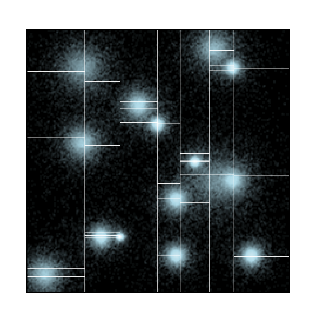
\includegraphics[width=8cm]{figure/pm3d.eps}
  \end{center}
  \caption{Example of the domain decomposition. The division is $7
    \times 6$ in 2-dimension.}
  \label{fig:decomposition}
\end{figure}


In the sampling method, first each process performs random sampling of
particles under it, and sends them to the process with rank 0
(``root'' process hereafter). Then the root process calculates the
division so that sample particles are equally divided over all
processes, and broadcasts the geometry of domains to all other
processes. In order to achieve good load balance, sampling frequency
should be changed according to the calculation cost per particle
\citep{2009PASJ...61.1319I}.

The sampling method works fine, if the number of particles per process
is significantly larger than the number of process. This is, however,
not the case for runs with a large number of nodes.  When the number
of particles per process is not much larger than the number of
processes, the total number of sample particles which the root process
needs to handle exceeds the number of particles per process itself,
and thus calculation time of domain decomposition in the root process
becomes visible.

%For example, K computer has more than 80,000 nodes, and in this paper
%we report the result of runs with all nodes. Even with Even with the
%number of particles per process same as the number of nodes, the
%total number of particles becomes 6.4 billion, and we do want to run
%simulations with smaller number of particles.

In order to reduce the calculation time, we also parallelized the
domain decomposition, currently in the direction of $x$ axis only. The
basic idea is that each node sends the sample particles not to the
root process of the all MPI processes but to the processes with index
$(i,0,0)$. Then processes $(i,0,0)$ sort the sample particles and
exchange the number of sample particles they received. Using these two
pieces of information, each of $(i,0,0)$ processes can determine all
domain boundaries inside its current domain in the $x$ direction. Thus,
they can determine which sample particles should be sent to
where. After the exchange of sample particles, each of $(i,0,0)$
processes can determine the decompositions in $y$ and $z$ directions.

A naive implementation of the above algorithm requires ``global''
sorting of sample particles over all of $(i,0,0)$ processes. In order
to simplify this part, before each process sends the sample particles
to  $(i,0,0)$ processes, they exchange their samples with other
processes with the same location in $y$ and $z$ process coordinates, so
that they have sample particles in the current domain decomposition in
the x direction. As a result, particles sent to $(i,0,0)$ processes
are already sorted at the level of domains decomposition in $x$
direction, and we need only the  sorting within each of $(i,0,0)$
processes to obtain the globally sorted particles.

Thus, our implementation of parallelized domain decomposition
is as follows:

\begin{enumerate}
\item
Each process samples particles randomly from its own particles. In
order to achieve an optimal load balance, the sampling rate of
particles is changed so that it is proportional to the CPU time per
particle spent on that process \citep{2009PASJ...61.1319I}. FDPS
provides several options including this optimal
balance. \label{prcoc:sampling}

%%
\item
Each process exchanges the sample particles according to the current
domain boundary in the $x$ direction with the process with the same y
and z indices, so that they have sample particles in the current
domain decomposition in the $x$ direction.


\label{proc:commx}

%%
\item
Each process with index $(i,y,z)$ sends the sample particles to the
process with index $(i,0,0)$, in other words, the root processes in
each of $y$-$z$ planes collects subsamples.

\label{proc:gatherx}

%%
\item
Each root process sorts the sample particles in the $x$ direction. Now,
the sample particles are sorted globally in the $x$ direction.

%%
\item
Each root process sends the number of the sample particles to the
other root processes and determines the global rank of the sample
particles.

%%
\item
Determine the $x$ coordinate of new domains by dividing all sample
particles into $n_x$ subsets with equal number of sample particles.
\label{proc:determinex}

%%
\item
Each root process exchanges sample particles with other root
processes, so that they have the sample particles in new domain in the
$x$ direction.

%\ref{proc:determinex}.

%of which $x$ coordinate is in the range of
%the $x$ coordinate of new subdomain determined in
%step

%%
\item
Each root process determines the $y$ and $z$ coordinates of new domains.
\label{proc:detyz}

%%
\item
Each root process broadcasts the geometries of new domains to all
other processes.
\label{proc:broadcasting}

\end{enumerate}

It is also possible to parallelize  the determination of  subdomains in
step \ref{proc:detyz}, but even for the full-node runs on K computer
we found the current parallelization is sufficient.

For particle exchange and also for interaction information exchange,
we use {\tt MPI\_Alltoall} to exchange the length of the data and {\tt
MPI\_Isend} and {\tt MPI\_Irecv} to actually exchange the data. At
least on K computer, we found that the performance of vendor-provided
{\tt MPI\_Alltoall} is not optimal for short messages. We implemented
a hand-crafted version in which the messages sent to the same relay
points are combined in order to reduce the total number of messages.


After the domain decomposition is done and the result is broadcasted
to all processes, they exchange particles so that each of them has
particles in its domain. Since each process has the complete
information of the domain decomposition, this part is pretty
straightforward to implement. Each process looks at each of its
particles, and determines if that particle is still in its domain.  If
not, the process determines to which process that particle should be
sent. After the destinations of all particles are determined, each
process sends them out, using {\tt MPI\_Isend} and {\tt MPI\_Irecv}
functions.


% LocalWords:  FDPS subdomain MPI multi subdomains DomainInfo ParticleSystem
% LocalWords:  decomposeDomainAll exchangeParticle substeps scalability
% LocalWords:  broadcasted Alltoallv
